\documentclass{beamer}
\mode<presentation>
\usepackage{amsmath}
\usepackage{amssymb}
%\usepackage{advdate}
\usepackage{adjustbox}
\usepackage{subcaption}
\usepackage{enumitem}
\usepackage{multicol}
\usepackage{mathtools}
\usepackage{listings}
\usepackage{url}
\def\UrlBreaks{\do\/\do-}
\usetheme{Boadilla}
\usecolortheme{lily}
\setbeamertemplate{footline}
{
  \leavevmode%
  \hbox{%
  \begin{beamercolorbox}[wd=\paperwidth,ht=2.25ex,dp=1ex,right]{author in head/foot}%
    \insertframenumber{} / \inserttotalframenumber\hspace*{2ex} 
  \end{beamercolorbox}}%
  \vskip0pt%
}
\setbeamertemplate{navigation symbols}{}

\providecommand{\nCr}[2]{\,^{#1}C_{#2}} % nCr
\providecommand{\nPr}[2]{\,^{#1}P_{#2}} % nPr
\providecommand{\mbf}{\mathbf}
\providecommand{\pr}[1]{\ensuremath{\Pr\left(#1\right)}}
\providecommand{\qfunc}[1]{\ensuremath{Q\left(#1\right)}}
\providecommand{\sbrak}[1]{\ensuremath{{}\left[#1\right]}}
\providecommand{\lsbrak}[1]{\ensuremath{{}\left[#1\right.}}
\providecommand{\rsbrak}[1]{\ensuremath{{}\left.#1\right]}}
\providecommand{\brak}[1]{\ensuremath{\left(#1\right)}}
\providecommand{\lbrak}[1]{\ensuremath{\left(#1\right.}}
\providecommand{\rbrak}[1]{\ensuremath{\left.#1\right)}}
\providecommand{\cbrak}[1]{\ensuremath{\left\{#1\right\}}}
\providecommand{\lcbrak}[1]{\ensuremath{\left\{#1\right.}}
\providecommand{\rcbrak}[1]{\ensuremath{\left.#1\right\}}}
\theoremstyle{remark}
\newtheorem{rem}{Remark}
\newcommand{\sgn}{\mathop{\mathrm{sgn}}}
\providecommand{\abs}[1]{\left\vert#1\right\vert}
\providecommand{\res}[1]{\Res\displaylimits_{#1}} 
\providecommand{\norm}[1]{\lVert#1\rVert}
\providecommand{\mtx}[1]{\mathbf{#1}}
\providecommand{\mean}[1]{E\left[ #1 \right]}
\providecommand{\fourier}{\overset{\mathcal{F}}{ \rightleftharpoons}}
%\providecommand{\hilbert}{\overset{\mathcal{H}}{ \rightleftharpoons}}
\providecommand{\system}{\overset{\mathcal{H}}{ \longleftrightarrow}}
	%\newcommand{\solution}[2]{\textbf{Solution:}{#1}}
%\newcommand{\solution}{\noindent \textbf{Solution: }}
\providecommand{\dec}[2]{\ensuremath{\overset{#1}{\underset{#2}{\gtrless}}}}
\newcommand{\myvec}[1]{\ensuremath{\begin{pmatrix}#1\end{pmatrix}}}
\let\vec\mathbf

\lstset{
%language=C,
frame=single, 
breaklines=true,
columns=fullflexible
}


\title{Presentation Template}
\author{Mokshith Kumar Reddy \\ Dept. of Electrical Engg.,\\IIT Hyderabad.}

\date{\today} 
\begin{document}

\begin{frame}
\titlepage
\end{frame}

\section*{Outline}
\section{Problem}
\begin{frame}
\frametitle{Question: }
    Using integration, find the area of the smaller region enclosed by the curve $4x^2 + 4y^2 = 9$ and the line $2x + 2y = 3$.\hfill{9.3.18}
\end{frame}
\section{Table}
\begin{frame}
\frametitle{Table for Reference}
\begin{table}[h]
    \centering
    \begin{tabular}{|c|c|}
        \hline
        Point & Coordinates\\
        \hline
        $A$ & \myvec{0\\6}\\
        \hline
        $B$ & \myvec{8\\0}\\
        \hline
        $C$ & \myvec{0\\0}\\
        \hline
\end{tabular}

    \caption{Parameters used}
    \label{}
\end{table}
\end{frame}
\section{Solution}
\subsection{Conic Parameters}
\begin{frame}
\frametitle{Given Parameters of Conics}
The given circle can be expressed as conics with parameters,
\begin{align}
    V=\myvec{4 & 0\\0 & 4}, u=0, f=-9.
\end{align}
The line parameters are:
\begin{align}
    h=\myvec{0\\ \frac{3}{2}}, m=\myvec{1\\-1}.
\end{align}
\end{frame}
\subsection{Theory}
\begin{frame}
\frametitle{Formulae for Finding Point of Intersection}
The points of intersection of the line 
\begin{align}
L: \quad x = h + \kappa m \quad \kappa \in \mathbb{R}
\end{align}
with the conic section 
\begin{align}
    \text{g}\brak{x} = x^{\top}Vx + 2u^{\top}x + f = 0
\end{align}
are given by
\begin{align}
x_i = h + \kappa_i m
\end{align}
where,
\begin{multline}
\kappa_i = \frac{1}{m^{\top}Vm} \left( -m^{\top}(Vh+u) \right) \\
\pm \sqrt{
\left( m^{\top}(Vh+u) \right)^2 - g(h) \cdot (m^{\top}Vm)
}
\end{multline}
\end{frame}
\subsection{Solving}
\begin{frame}
\frametitle{Finding Area of intersection}
Substituting the parameters in the above equation yields:
\begin{align}
    k=0,\frac{3}{2}.
\end{align}
This gives the points of intersection as:
\begin{align}
    A=\myvec{\frac{3}{2}\\0}, B=\myvec{0\\ \frac{3}{2}}.
\end{align}
The desired area is:
\begin{align}
\int_{0}^{\frac{3}{2}}\frac{\sqrt{9-4x^2}}{2}-\int_{0}^{\frac{3}{2}}\frac{3-2x}{2}=\frac{9}{16}\pi-\frac{9}{8}.
\end{align}
\end{frame}
\section{Plot}
\begin{frame}
\frametitle{Figure}
\begin{figure}[h!]
   \centering
   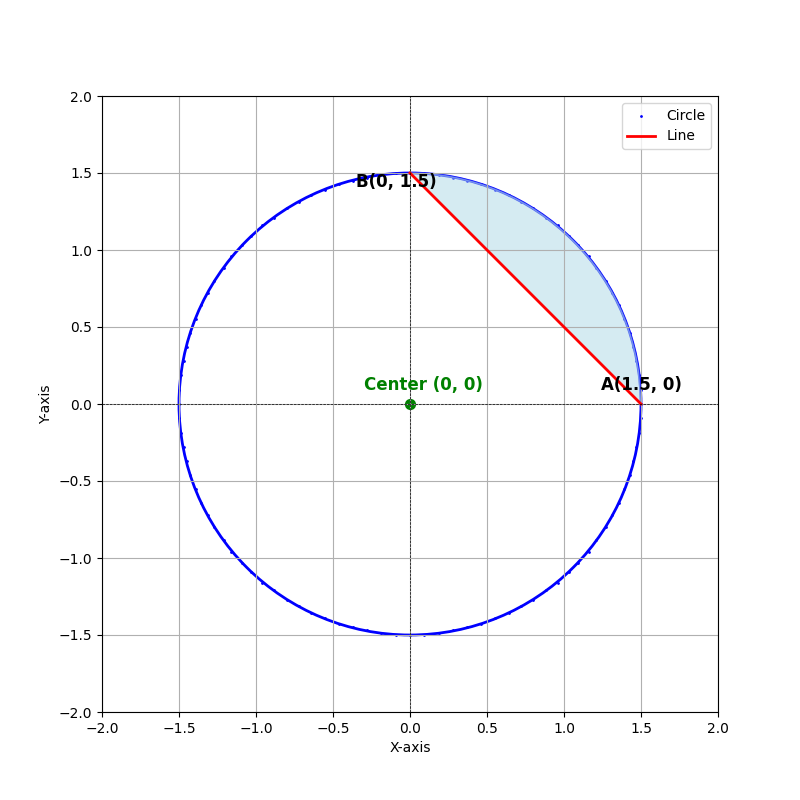
\includegraphics[width=0.7\linewidth]{figs/plot.png}
   \caption{ }
   \label{plot}
\end{figure}
\end{frame}
\section{code}
\begin{frame}
\frametitle{Code for Finding Points}
\begin{figure}[h!]
   \centering
   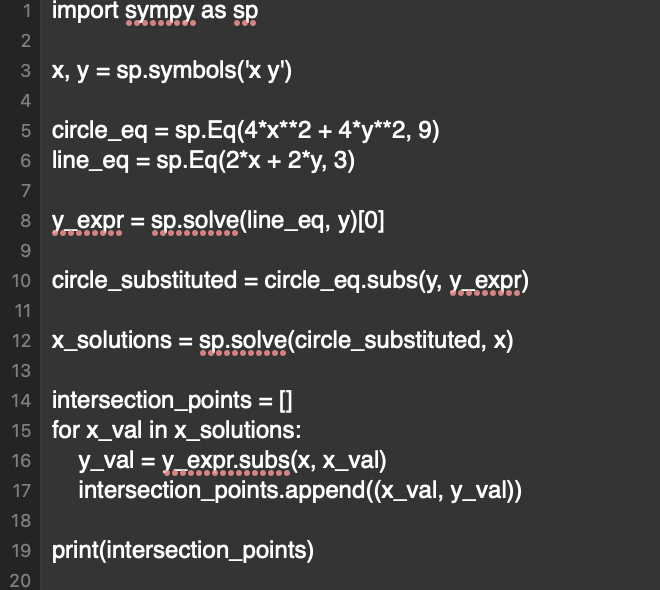
\includegraphics[width=0.7\linewidth]{figs/fig2.png}
   \caption{ }
   \label{code}
\end{figure}
\end{frame}
\end{document}
